\documentclass{beamer}

\usepackage{default}
\usepackage[utf8]{inputenc}
\usepackage[T1]{fontenc}
%\usepackage[ngerman]{babel}
\usepackage{enumerate}
\usepackage{listings}
\usepackage{marvosym}
\usepackage{gensymb}
\usepackage{graphicx}

\graphicspath{{./img/}}

\usetheme{Pittsburgh}
\usecolortheme{seagull}


\title{B.Sc. Thesis Exposé}
\subtitle{\it Megamodel-driven Traceability Recovery \& Exploration of Correspondence \& Conformance Links}
\author{Maximilian Meffert\\~(210~101~205)}
\institute{University of Koblenz-Landau}
\date{}

\beamertemplatenavigationsymbolsempty 
\setbeamertemplate{bibliography item}[text]

\makeatother
\setbeamertemplate{footline}[text line]{
\parbox{\linewidth}{
\vspace*{-8pt}
\tiny
\insertshorttitle
\hfill
\insertshortauthor
\hfill
\insertshortinstitute
\hfill
}}
\makeatletter

\newcommand{\partOf}{~\textsf{partOf}~}
\newcommand{\properPartOf}{~\textsf{properPartOf}~}
\newcommand{\Any}{~\textsf{Any}~}
\newcommand{\correspondsTo}{~\textsf{correspondsTo}~}
\newcommand{\correspondsToR}[1]{~\textsf{correspondsTo}_{#1}~}
\newcommand{\conformsTo}{~\textsf{conformsTo}~}


\newcommand{\megal}{\text{MegaL}}
\newcommand{\megalxtext}{\text{MegaL/Xtext}}
\newcommand{\megaltext}{\text{MegaL/Text}}
\newcommand{\eclipse}{\text{eclipse}}

\begin{document}

\frame{\titlepage}

\begin{frame}[allowframebreaks]{Motivation}
\begin{center}
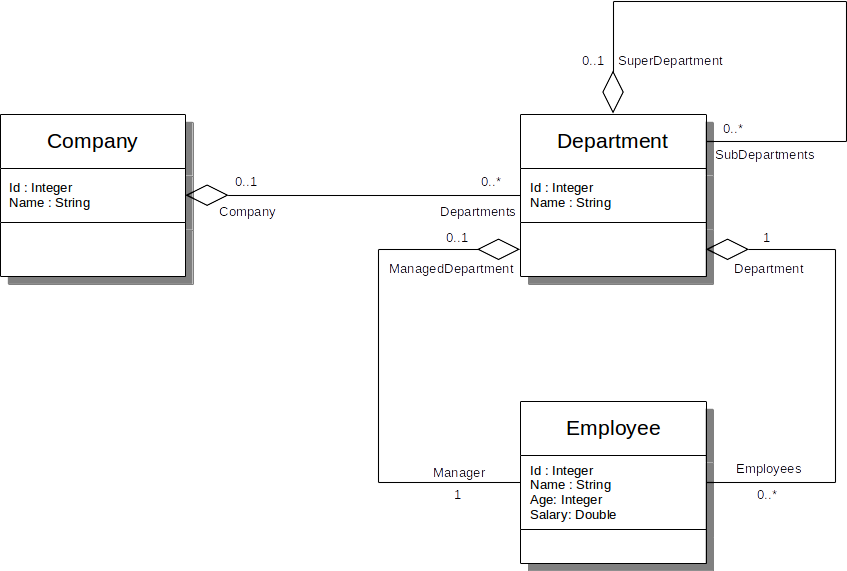
\includegraphics[width=.6\textwidth]{companies.png}
\newline
\scriptsize
The \textit{101companies} Human Resources Management System
\end{center}
Given an application-/domain-model, it can be ...
\begin{itemize}
\item ... \textbf{serialized}, e.g. to XML
\item ... \textbf{persisted}, e.g. into a relational database
\end{itemize}
\newpage
\begin{center}
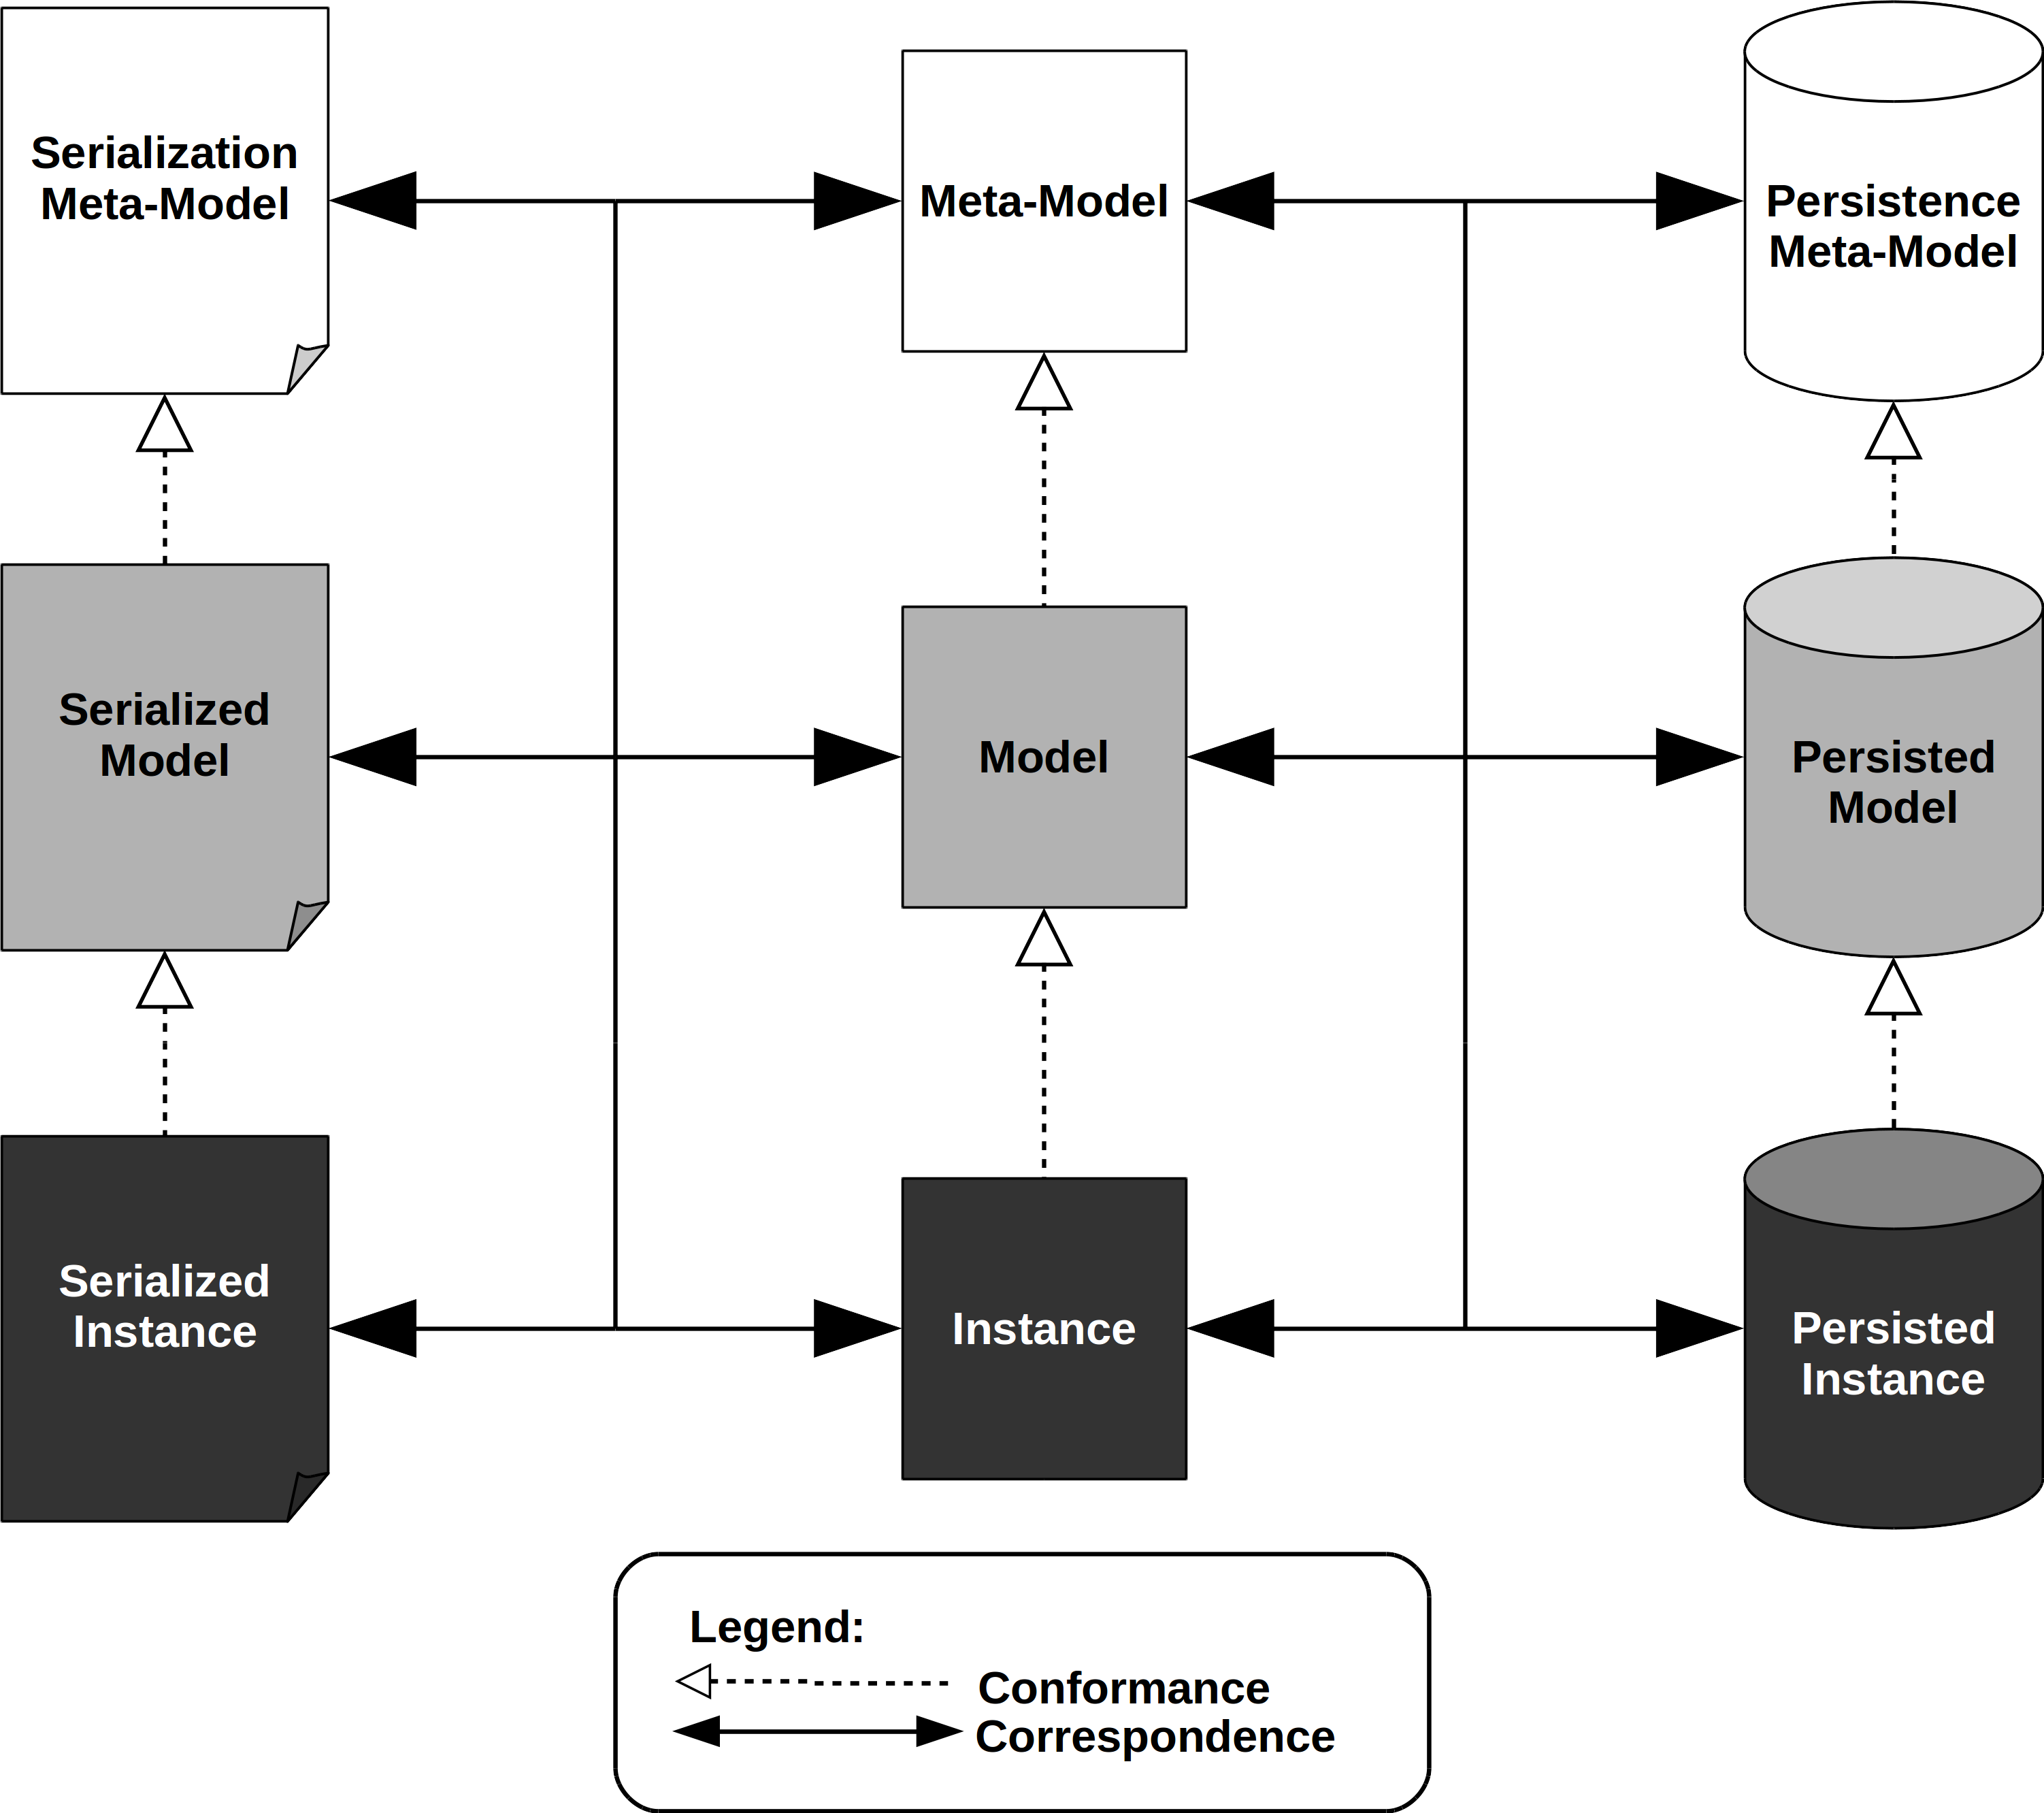
\includegraphics[width=.7\textwidth]{orx-cc-scenario.png}
\newline
O/R/X Correspondence \& Conformance Scenario
\end{center}
\newpage
\begin{center}
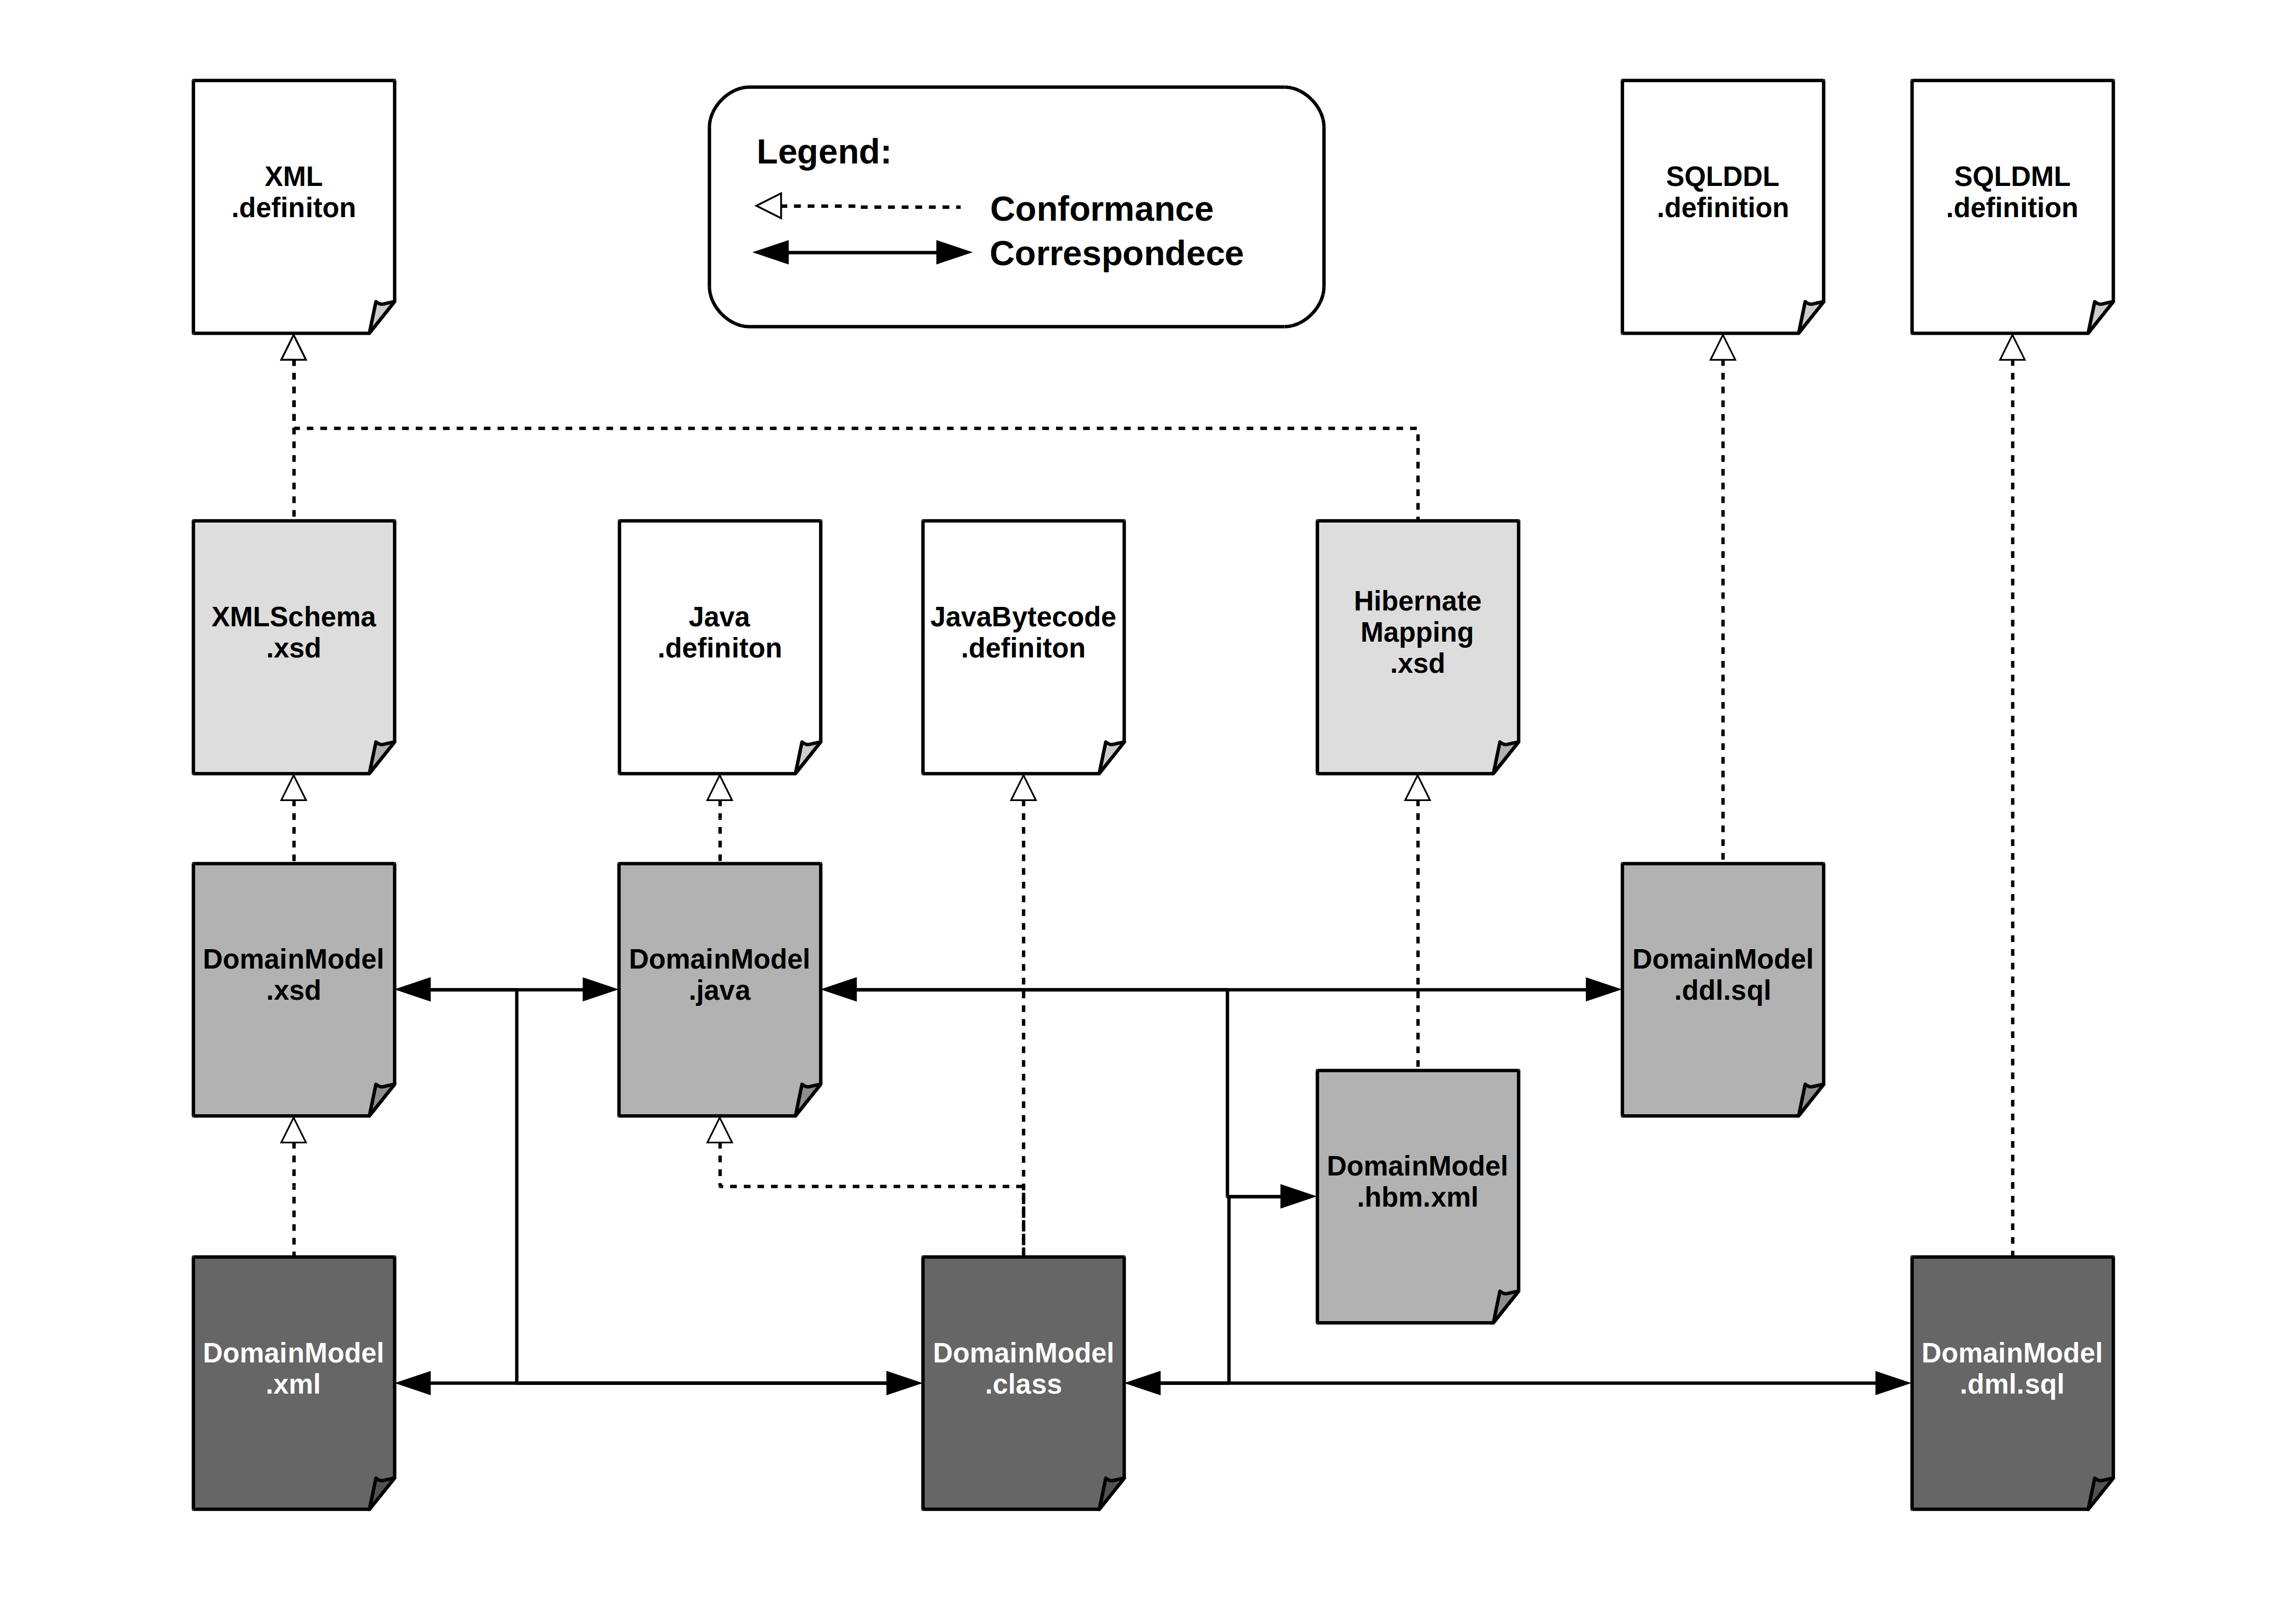
\includegraphics[width=.9\textwidth]{orx-correspondence-big-picture.png}
\newline
O/R/X Correspondence \& Conformance Artifact Links
\end{center}
\end{frame}

\begin{frame}{Formal Background}
\begin{itemize}
\item
\textbf{Parthood/Mereology}\cite{DBLP:conf/sle/Lammel16}\cite{DBLP:journals/dke/Varzi96}
{\scriptsize
\begin{align*}
&x \partOf x
\\&x \partOf y \wedge y \partOf x \Rightarrow x = y
\\&x \partOf y \wedge y \partOf z \Rightarrow x \partOf z
\\&x \properPartOf y \Leftrightarrow x \partOf y \wedge \neg(y \partOf x)
\end{align*}
}
\item
\textbf{Correspondence}\cite{DBLP:conf/sle/Lammel16}
{\scriptsize
\begin{align*}
&(a_1,a_2) \in R \subseteq L_1 \times L_2
\\&\wedge \forall b_1 \in L_1 : b_1 \partOf a_1 \Rightarrow (\exists! b_2 \in L_2 : b_2 \partOf a_2 \wedge b_1 \correspondsToR{R} b_2 )
\\&\wedge \forall b_2 \in L_2 : b_2 \partOf a_2 \Rightarrow (\exists! b_1 \in L_1 : b_1 \partOf a_2 \wedge b_2 \correspondsToR{R} b_1 )
\\&\Rightarrow a_1 \correspondsToR{R} a_2
\end{align*}
}
\item
\textbf{Conformance}\cite{DBLP:conf/sle/Lammel16}
{\scriptsize
\begin{align*}
\forall x \in \Any :
x \in L \subseteq \Any \Leftrightarrow \exists d \in D \subseteq \Any : x \conformsTo d
\end{align*}
}

\end{itemize}
\end{frame}

\begin{frame}{Research Hypotheses}
\begin{enumerate}[RH1]
\item
\textbf{Fragment Correspondence Hypothesis}
{\scriptsize
\begin{align*}
&\forall a_1 \in L_1, a_2 \in L_2 \exists b_1 \in L_1, b_2 \in L_2 :  
\\&a_1 \correspondsToR{R} a_2
\Rightarrow 
b_1 \partOf a_2 
\wedge b_2 \partOf a_2
\wedge b_1 \correspondsToR{R} b_2
\end{align*}
}
\item
\textbf{Fragment Conformance Hypothesis}
{\scriptsize
\begin{align*}
&\forall a_1 \in L, a_2 \in D \exists b_1 \in L, b_2 \in D : 
\\&a_1 \conformsTo a_2
\Rightarrow 
b_1 \partOf a_2
\wedge b_2 \partOf a_2
\wedge b_1 \conformsTo b_2
\end{align*}
}
\end{enumerate}
\begin{center}
\tiny
Note, these hypotheses may be problematic / to weak,
\\because parthood is reflexive they are inherently true.
\end{center}
\end{frame}

\begin{frame}{Research Questions}
\begin{enumerate}[RQ1]

\item
\textbf{Is correspondence to some extend strictly mereologically induced?}
{\scriptsize
\begin{align*}
&\forall a_1 \in L_1, a_2 \in L_2 \exists b_1 \in L_1, b_2 \in L_2 :
\\&a_1 \correspondsToR{R} a_2
\\&\Rightarrow 
b_1 \properPartOf a_2 
\wedge b_2 \properPartOf a_2 
\wedge b_1 \correspondsToR{R} b_2
\end{align*}
}

\item
\textbf{Is conformance to some extend strictly mereologically induced?}
{\scriptsize
\begin{align*}
&\forall a_1 \in L_1, a_2 \in L_2 \exists b_1 \in L_1, b_2 \in L_2 :
\\&a_1 \conformsTo a_2
\\&\Rightarrow 
b_1 \properPartOf a_2 
\wedge b_2 \properPartOf a_2 
\wedge b_1 \conformsTo b_2
\end{align*}
}

\end{enumerate}
\end{frame}

\begin{frame}{Thesis Objectives}
\small
\begin{enumerate}[TO1]
\item
Implementation of a $\megalxtext$-extension capable of recovering traceability links representing parthood, correspondence and conformance relationships between code fragments.

\item
Implementation of a $\megalxtext$-extension allowing for an user to visually explore traceability links, i.e. parthood, correspondence and conformance relationships between code fragments

\item
Providing an extensive discussion comparing $\megal$\cite{DBLP:conf/models/FavreLV12} with related approaches on traceability recovery.

\item
Providing an extensive discussion comparing $\megal$\cite{DBLP:conf/models/FavreLV12} with related approaches on ontologies for software artifacts or software engineering in general.

\item
Providing an answer for the research questions.
\end{enumerate}
\end{frame}

\begin{frame}[allowframebreaks]{References}
\scriptsize{\bibliographystyle{plain}}
\bibliography{../bsc}{}
\end{frame}


\end{document}
